%%%%% Code to convert a Tikz picutre to a standalone picutre file %%%%%
%%%%% See for more information: https://hh360.user.srcf.net/blog/2015/04/converting-from-tikz-to-png/ %%%%%
% Example command for PNG creation: pdflatex --shell-escape Tikz_picture_to_PNG.tex
\documentclass[preview,border=4mm,convert={density=600,outext=.png}]{standalone}

\usepackage{url}
\usepackage{tikz}
\usepackage{color}
\begin{document}

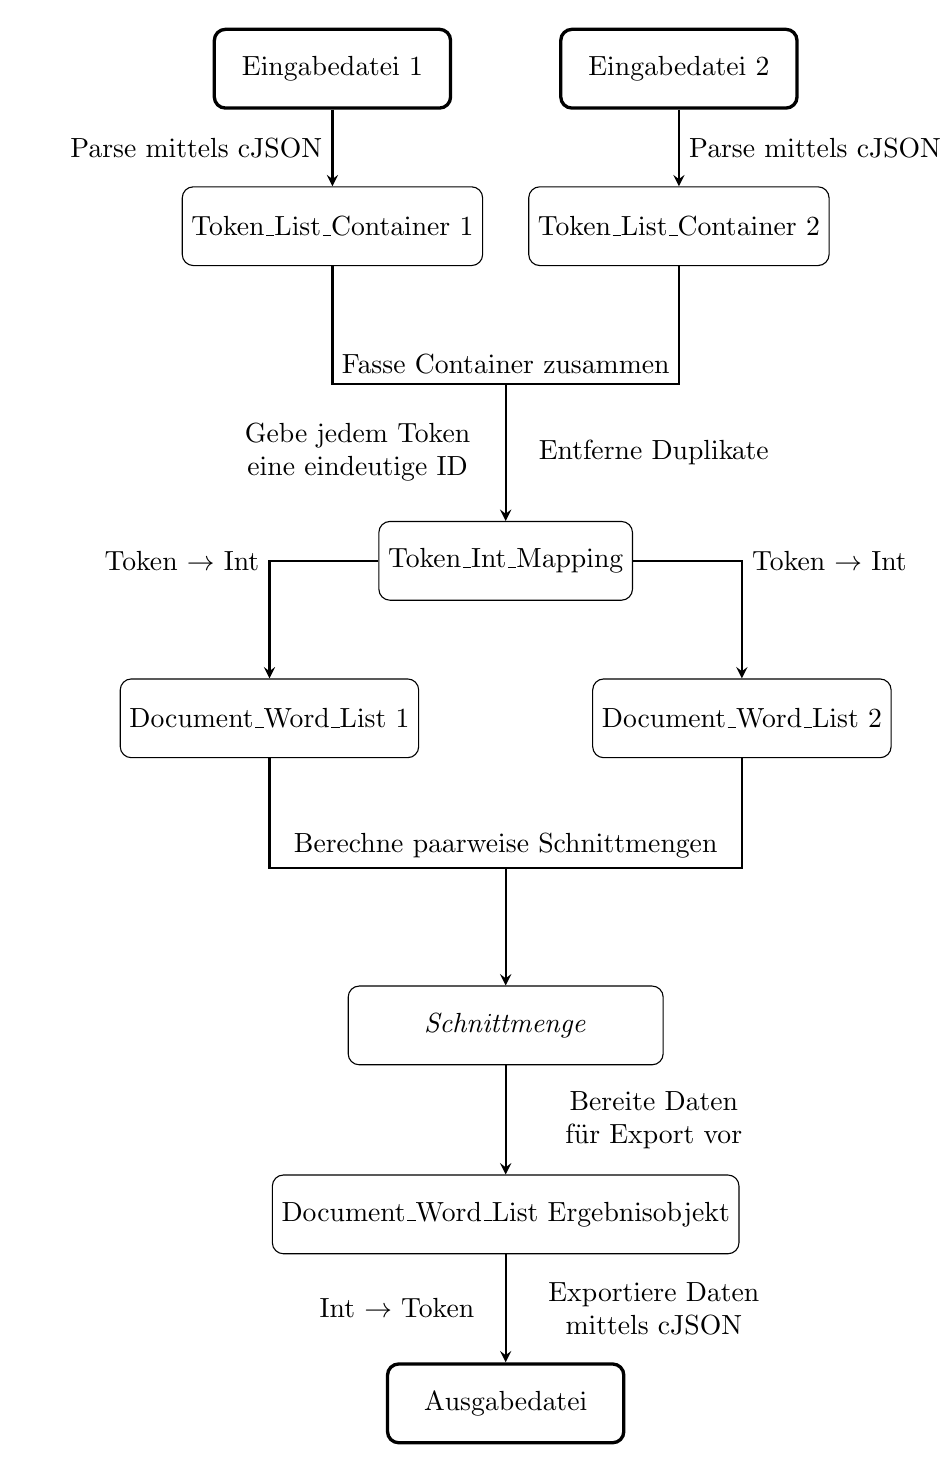
\begin{tikzpicture}[node distance=2cm]
    % Centering the picutre (This value maybe need to be adjusted, when the picutre was changed)
    \hspace*{0.425cm}

    \tikzstyle{in_out} = [rectangle, rounded corners, minimum width=3cm, minimum height=1cm, text centered, draw=black, very thick]%, fill=red!30]
    \tikzstyle{rect} = [rectangle, rounded corners, minimum width=3cm, minimum height=1cm, text centered, draw=black]
    \tikzstyle{process} = [rectangle, rounded corners, minimum width=0.75cm, minimum height=0.75cm,text centered, draw=black, fill=gray!12.5]
    \tikzstyle{intersection} = [rectangle, rounded corners, minimum width=4cm, minimum height=1cm, text centered, draw=black]
    \tikzstyle{arrow} = [thick,->,>=stealth]

            % node[Optionen](Name){Inhalt}
            \node (Eingabedatei1) [in_out, xshift=0cm] {Eingabedatei 1};
            \node (Eingabedatei2) [in_out, xshift=4.4cm] {Eingabedatei 2};

            \node (Token_List_Container1) [rect, below of=Eingabedatei1] {Token\_List\_Container 1};
            \node (Token_List_Container2) [rect, below of=Eingabedatei2] {Token\_List\_Container 2};

            \node (Inv1) [coordinate, below of=Token_List_Container1, xshift=2.2cm, yshift=-0cm, label=Fasse Container zusammen] {};

            \node (Token_Int_Mapping) [rect, below of=Inv1, yshift=-0.25cm] {Token\_Int\_Mapping};
            \node (Document_Word_List1) [rect, below of=Token_Int_Mapping, xshift=-3cm] {Document\_Word\_List 1};
            \node (Document_Word_List2) [rect, below of=Token_Int_Mapping, xshift=3cm] {Document\_Word\_List 2};

            \node (Inv2) [coordinate, below of=Document_Word_List1, xshift=3cm, yshift=0.1cm, label=Berechne paarweise Schnittmengen] {};
            \node (Intersection) [intersection, below of=Inv2, yshift=0.0cm] {\emph{Schnittmenge}};
            \node (Document_Word_List_Ergebnis) [rect, below of=Intersection, yshift=-0.4cm] {Document\_Word\_List Ergebnisobjekt};

            \node (Ausgabedatei) [in_out, below of=Document_Word_List_Ergebnis, yshift=-0.4cm] {Ausgabedatei};

            % ----- ----- ----- ----- ----- ----- ----- ----- ----- ----- ----- ----- ----- ----- ----- ----- ----- ----- -----

            \draw [arrow] (Eingabedatei1) -- node[anchor=east] {Parse mittels cJSON} (Token_List_Container1);
            \draw [arrow] (Eingabedatei2) -- node[anchor=west] {Parse mittels cJSON} (Token_List_Container2);
            \draw [thick] (Token_List_Container1) |- (Inv1);
            \draw [thick] (Token_List_Container2) |- (Inv1);
            \draw [arrow] (Inv1) -- node[anchor=west, text centered, text width=3.5cm]{Entferne Duplikate} node[anchor=east, text centered, text width=3.5cm]{Gebe jedem Token eine eindeutige ID} (Token_Int_Mapping);
            \draw [arrow] (Token_Int_Mapping) -| node[anchor=east] {Token $ \rightarrow $ Int} (Document_Word_List1);
            \draw [arrow] (Token_Int_Mapping) -| node[anchor=west] {Token $ \rightarrow $ Int} (Document_Word_List2);
            \draw [thick] (Document_Word_List1) |- (Inv2);
            \draw [thick] (Document_Word_List2) |- (Inv2);
            \draw [arrow] (Inv2) -- (Intersection);
            \draw [arrow] (Intersection) -- node[anchor=west, text centered, text width=3.5cm] {Bereite Daten für Export vor} (Document_Word_List_Ergebnis);
            \draw [arrow] (Document_Word_List_Ergebnis) -- node[anchor=east, text centered, text width=2.5cm] {Int $ \rightarrow $ Token} node[anchor=west, text centered, text width=3.5cm] {Exportiere Daten mittels cJSON} (Ausgabedatei);
\end{tikzpicture}

\end{document}
